\subsubsection{Redux} \label{subsection:4-2-2-2-redux}

\logo{chapter-4/4.2.redux-logo}{Redux logo}

Το Redux\footnote{\url{https://redux.js.org/}} αποτελεί μία βιβλιοθήκη JavaScript, η χρήση της οποίας προσφέρει στην εφαρμογή ένα πλήρως διαχειρίσιμο global state.

Τα δομικά στοιχεία του Redux είναι τα εξής:
\begin{itemize}
	\item \textbf{Actions}: Αντικείμενα τα οποία περιέχουν νέα πληροφορία για την τροποποίηση του state της εφαρμογής.
	\item \textbf{Reducers}: Συναρτήσεις οι οποίες λαμβάνοντας ένα action και διαβάζοντας το τρέχον state, εφαρμόζουν κάποια λογική για την παραγωγή ενός νέου state.
	\item \textbf{Store}: Το αντικείμενο στο οποίο βρίσκεται αποθηκευμένο το state της εφαρμογής. Η βασική ιδιότητα του state είναι ότι παραμένει αμετάβλητο και, για την ανανέωσή του, παράγεται πάντα ένα νέο state object μέσω των reducer.
	\item \textbf{Middleware}: Προαιρετικά κομμάτια κώδικα που λαμβάνουν actions πριν εκείνα φτάσουν στους reducers και εκτελούν κάποιο side effect. Συνήθως χρησιμοποιούνται για ενέργειες όπως logging και error reporting ή για να ενώσουν το Redux με εξωτερικά APIs. 
\end{itemize}

Αν και το ίδιο το Redux είναι μικροσκοπικό σε μέγεθος, ο τρόπος υλοποίησής του έχει επιτρέψει τη δημιουργία ενός τεράστιου οικοσυστήματος εργαλείων και επεκτάσεων, τα οποία συνδέονται μαζί του ή βασίζονται σε αυτό. Για παράδειγμα, μία από τις κύριες χρήσεις του είναι η κατασκευή διεπαφών χρήστη σε συνδύασμό με άλλες βιβλιοθήκες, όπως με την React. Σε αυτήν την περίπτωση, συνδέεται μαζί της με το npm πακέτο \texttt{react-redux} και η λειτουργία του υπό ανάπτυξη UI προκύπτει ως εξής:

%TODO: Add proper diagram
\begin{figure}[H]
	\centering
	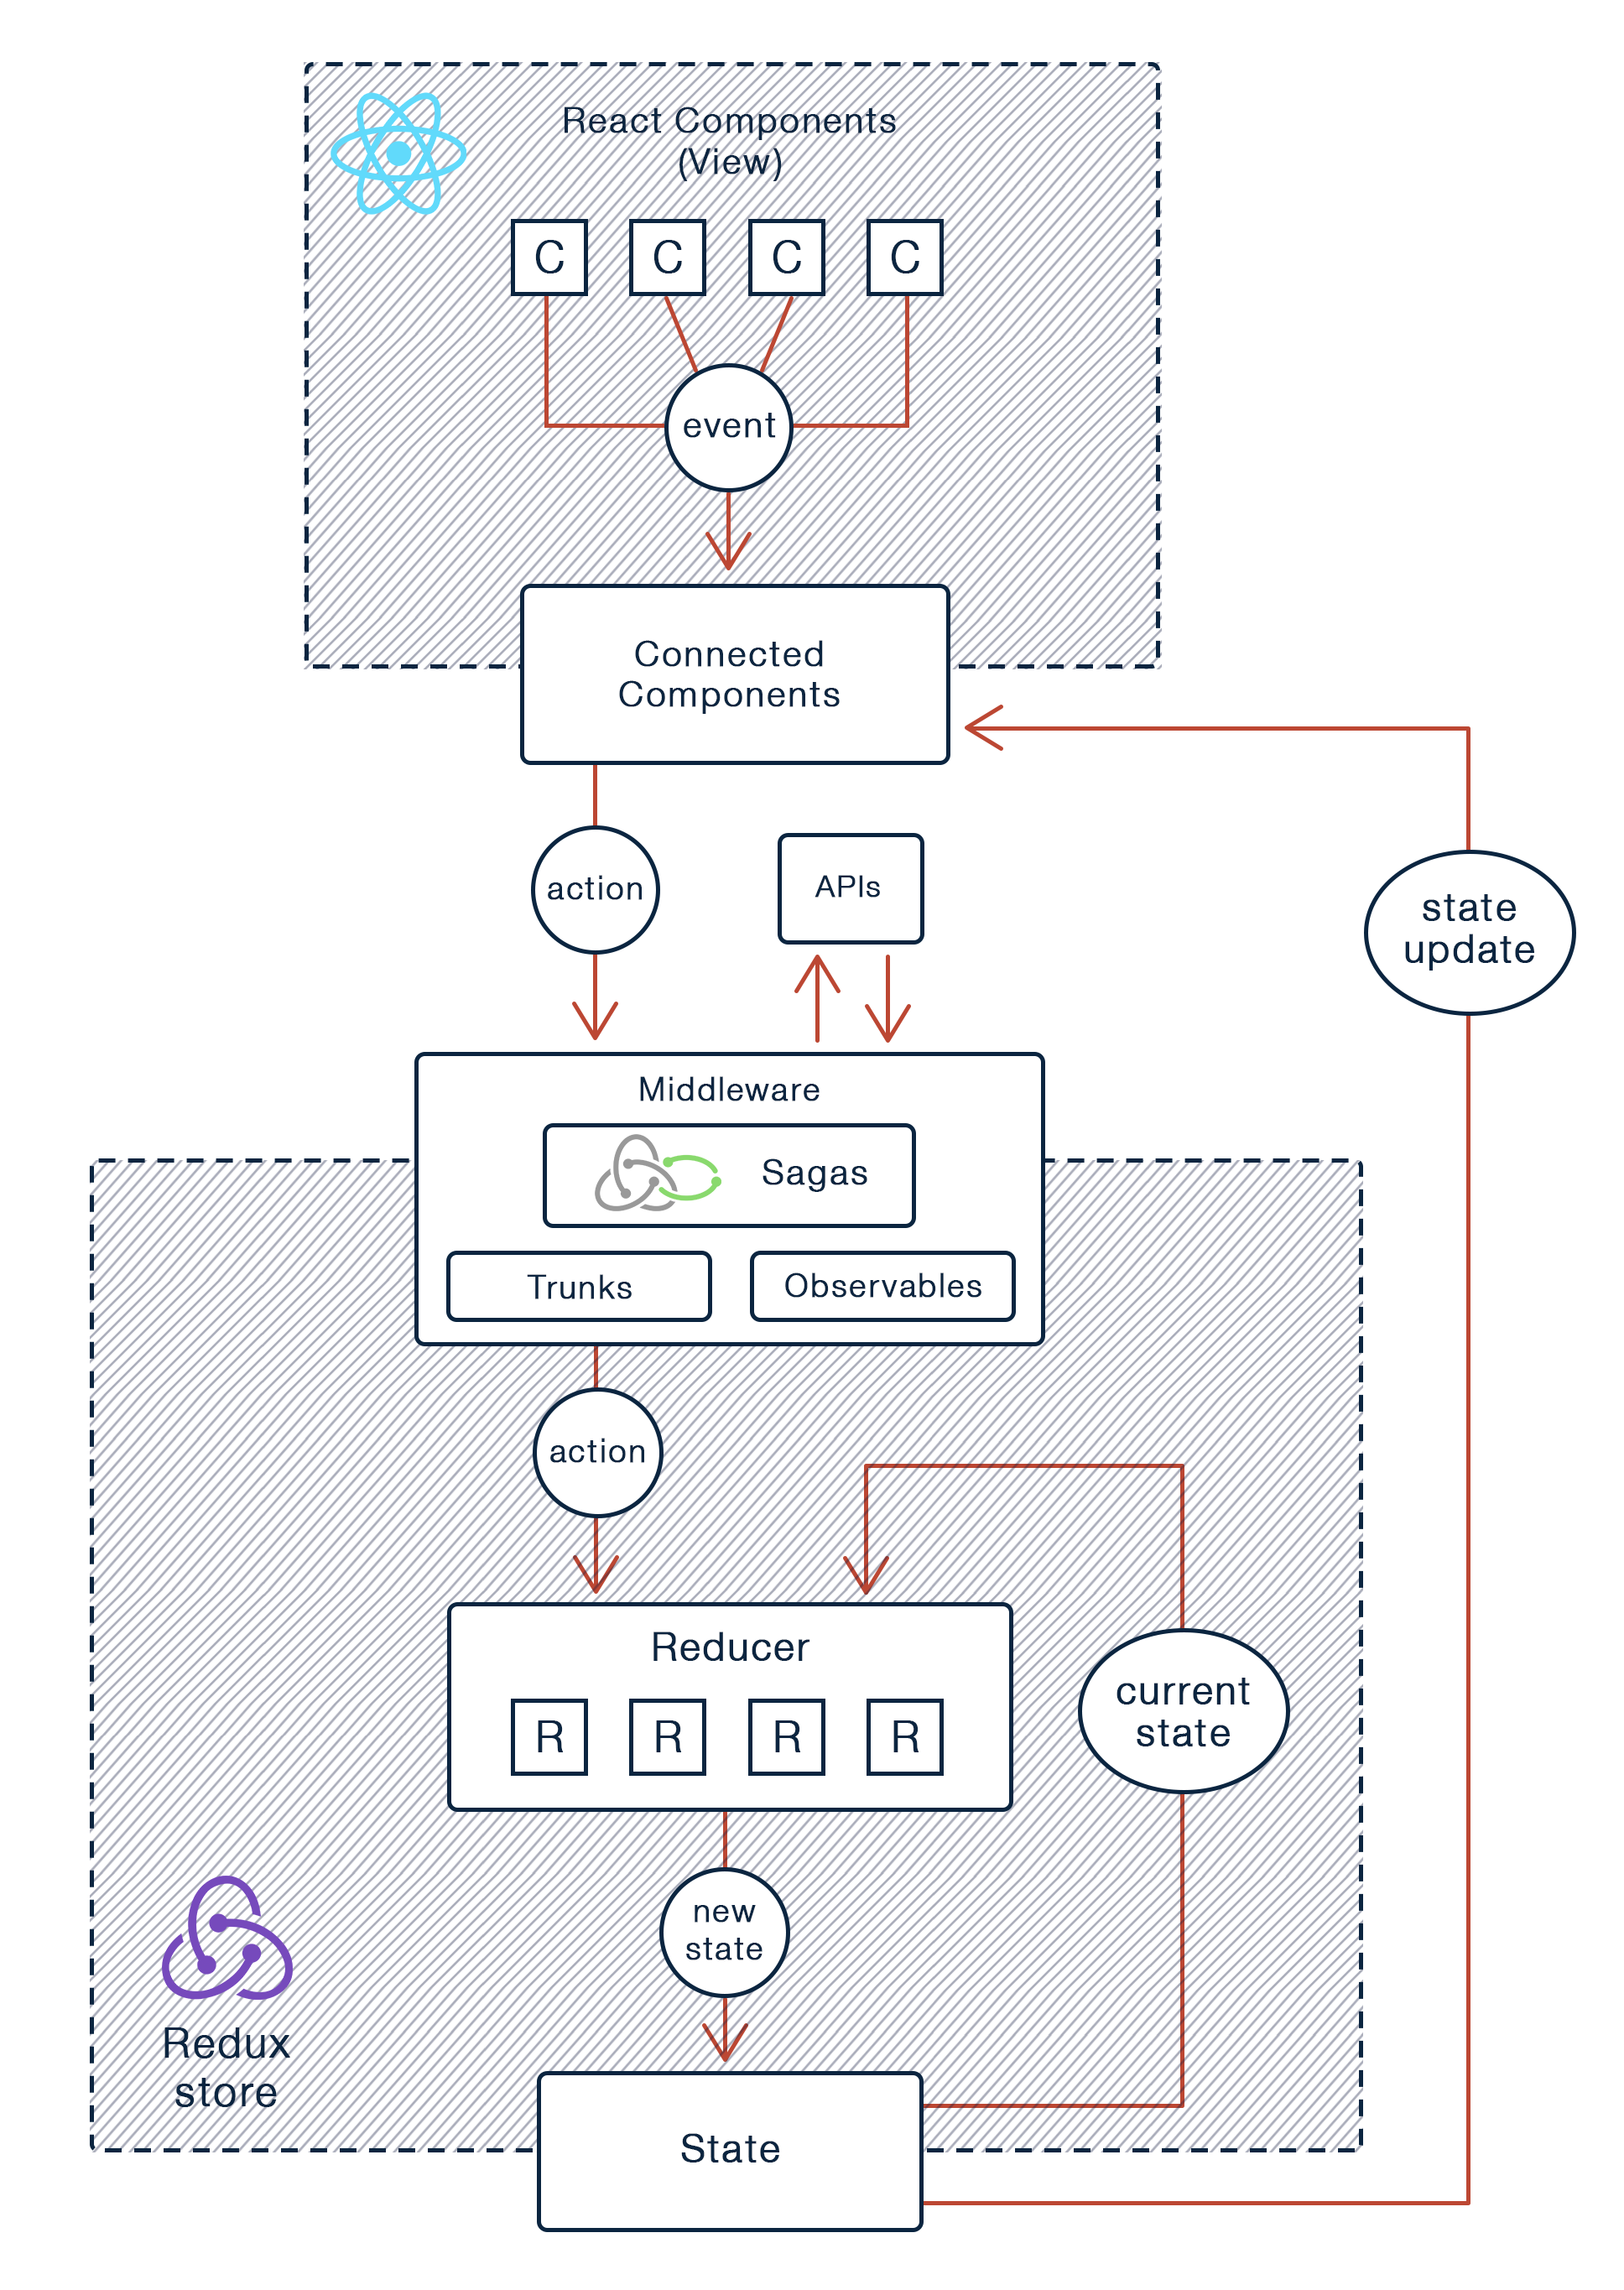
\includegraphics[width=.75\textwidth]{assets/figures/chapter-4/4.2.react-redux}
	\caption{Λειτουργία του Redux σε συνδυασμό με React}
\end{figure}

Το Redux έχει το αποθετήριό του στο GitHub (\url{https://github.com/reduxjs/redux}) και διατίθεται μέσω του μητρώου npm (\url{https://www.npmjs.com/package/redux}).
